\documentclass[11pt,a4paper]{article}
\newcommand{\guideshort}{Beginner quickstart}
% Shared typesetting for the two source-grounded VGAI teaching guides.
\usepackage[a4paper,margin=23mm,headheight=15pt]{geometry}
\usepackage{fontspec}
\setmainfont{Liberation Serif}
\setsansfont{Liberation Sans}
\setmonofont{Liberation Mono}
\usepackage{xcolor,graphicx,booktabs,tabularx,longtable,array}
\usepackage{listings,hyperref,tikz}
\usetikzlibrary{arrows.meta,positioning}
\definecolor{vveblue}{HTML}{174A70}
\definecolor{vvelight}{HTML}{F1F5F8}
\definecolor{vvegreen}{HTML}{266547}
\hypersetup{colorlinks=true,linkcolor=vveblue,urlcolor=vveblue,
  pdfauthor={Vienna Game AI Library},pdfsubject={Source-grounded beginner teaching edition}}
\setlength{\parindent}{0pt}
\setlength{\parskip}{6pt plus 1pt}
\setlength{\emergencystretch}{3em}
\sloppy
\renewcommand{\arraystretch}{1.18}
\makeatletter
\def\ps@vve{%
  \def\@oddhead{\small\sffamily Vienna Game AI Library\hfil\guideshort}%
  \let\@evenhead\@oddhead
  \def\@oddfoot{\small\sffamily Teaching edition / 16 October 2026\hfil\thepage}%
  \let\@evenfoot\@oddfoot}
\makeatother
\pagestyle{vve}
\lstdefinestyle{vvecpp}{language=C++,basicstyle=\ttfamily\small,
  keywordstyle=\color{vveblue}\bfseries,commentstyle=\color{vvegreen},
  stringstyle=\color{vvegreen},backgroundcolor=\color{vvelight},
  breaklines=true,breakatwhitespace=false,columns=fullflexible,
  keepspaces=true,showstringspaces=false,tabsize=4,
  frame=single,rulecolor=\color{vvelight},framesep=6pt,
  xleftmargin=6pt,xrightmargin=6pt,aboveskip=8pt,belowskip=8pt,
  morekeywords={import,requires,concept,constexpr,consteval,nodiscard}}
\lstset{style=vvecpp}
\newcommand{\api}[1]{{\ttfamily\small\detokenize{#1}}}
\newcommand{\source}[1]{\par\smallskip{\raggedright\footnotesize\sffamily\color{vveblue}Source: \nolinkurl{#1}.\par}}
\newcommand{\lesson}[1]{\clearpage\section{#1}}
\newenvironment{remember}{\begin{quote}\small\textbf{Remember. }}{\end{quote}}
\newenvironment{tryit}{\begin{quote}\small\textbf{Try it. }}{\end{quote}}
\newcommand{\guidecover}[3]{%
 \begin{titlepage}\sffamily\color{vveblue}
 {\large Vienna Game AI Library\par}\vspace{20mm}
 {\Huge\bfseries #1\par}\vspace{8mm}
 {\Large #2\par}\vspace{12mm}
 \color{black}{\large #3\par}\vfill
 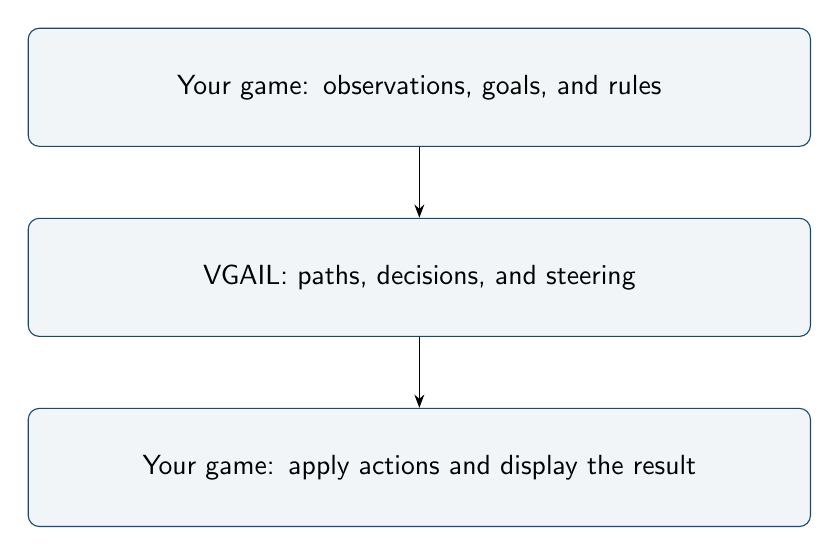
\begin{tikzpicture}[node distance=9mm,every node/.style={draw=vveblue,rounded corners,fill=vvelight,text width=0.8\linewidth,align=center,minimum height=15mm,font=\sffamily}]
 \node (game) {Your game: observations, goals, and rules};
 \node (engine) [below=of game] {VGAIL: paths, decisions, and steering};
 \node (result) [below=of engine] {Your game: apply actions and display the result};
 \draw[-{Stealth}] (game)--(engine);
 \draw[-{Stealth}] (engine)--(result);
 \end{tikzpicture}\vfill
 {\normalsize Updated 16 October 2026\par}
 {\small Source baseline: b1c76a1.\par}
 {\small Complete examples are checked against this source; excerpts state their context.\par}
 \end{titlepage}}

\hypersetup{pdftitle={Vienna Game AI Library - Beginner quickstart}}
\begin{document}
\guidecover{Beginner quickstart}{Routes, decisions and movement in small steps}{Start with console examples using the actual single-header library. No graphics setup or prior game AI knowledge is required.}
\tableofcontents
\lesson{What you are going to build}
VGAI is the Vienna Game AI Library. It supplies small algorithms for choosing actions, finding routes and moving agents. It is not a complete game engine. Your game still owns input, the world, collision handling and rendering.

The code is in one header, \api{include/ViennaGameAILibrary.hpp}. Its namespace is \api{VGAIL}, including the final L. You use a C++ \api{#include}; this project does not provide a C++ module named VGAI.

Start with a console program that finds a route across an eight-by-six grid. A grid cell is one square of a map. Its coordinates are whole numbers starting at zero. We will then add a state machine and a moving agent. The complete programs print success flags and return zero when their checks pass.

You need basic C++ variables, functions and loops. The longer guide explains vectors, pointers, callbacks and ownership as they appear. No knowledge of machine learning, neural networks or game-engine internals is needed.
\lesson{Build without graphics}
Create a game folder beside \api{ViennaGameAILibrary}. Save the next page's complete pathfinding program as \api{main.cpp}. Save this build file as \api{CMakeLists.txt}:\begin{lstlisting}
cmake_minimum_required(VERSION 3.20)
project(FirstAI LANGUAGES CXX)
find_package(Threads REQUIRED)
add_executable(first_ai main.cpp)
target_compile_features(first_ai PRIVATE cxx_std_20)
target_compile_definitions(first_ai PRIVATE NDEBUG)
target_include_directories(first_ai PRIVATE
    ../ViennaGameAILibrary/include)
target_link_libraries(first_ai PRIVATE Threads::Threads)
\end{lstlisting}
Then run:\begin{lstlisting}
cmake -S . -B build -DCMAKE_BUILD_TYPE=Release
cmake --build build
# Run build/first_ai on a single-configuration Linux build.
\end{lstlisting}
On a multi-configuration generator, build with \api{--config Release} and find the executable in its Release folder. On Linux or macOS you can also use a suitable compiler directly:\begin{lstlisting}
c++ -std=c++20 -DNDEBUG -pthread \
    -I../ViennaGameAILibrary/include main.cpp -o first_ai
./first_ai
\end{lstlisting}
The examples include a few standard headers before the library because the current header uses their declarations. \api{NDEBUG} avoids the current Windows-specific \api{__debugbreak()} assertion path on Linux. Check inputs in your program; do not rely on disabled assertions to reject them.

You do not need raylib for these console examples. The repository's top-level CMake always adds its graphical Demo. That route requires its raylib submodule; use it after the console exercise works.
\source{include/ViennaGameAILibrary.hpp; CMakeLists.txt; Demo/CMakeLists.txt}
\lesson{A complete pathfinding program}
% doc-example: vgai_path
\begin{lstlisting}
#include <cfloat>
#include <cmath>
#include <cstdint>
#include <limits>
#include "ViennaGameAILibrary.hpp"

int main() {
    VGAIL::NavMesh map(8, 6, 0.0f);
    map.setObstructable({3, 2});
    auto path = map.findPath({0, 0}, {7, 5});
    const bool ok = !path.empty()
        && path.front() == VGAIL::Vec2ui{0, 0}
        && path.back() == VGAIL::Vec2ui{7, 5};
    std::cout << "path ok=" << ok
              << " cells=" << path.size() << '\n';
    for (const auto& p : path)
        std::cout << p.x << ',' << p.y << '\n';
    return ok ? 0 : 1;
}
\end{lstlisting}
Expected result: \api{path ok=1}, a positive number of cells and a list from \api{0,0} to \api{7,5}. Do not require one exact route if several routes have equal cost. The third constructor argument is the randomly obstructed fraction. Zero makes the initial grid entirely walkable; we then block one cell explicitly.

The route includes the start and target. Empty output means no route was found. A request from a walkable cell to itself returns that cell. Check bounds and walkability before requesting a route; the current implementation does not provide a checked-result wrapper for invalid coordinates.
\lesson{Understand the route before moving anything}
Although the class is called \api{NavMesh}, this implementation represents a rectangular grid. Coordinates use \api{Vec2ui}: two unsigned whole numbers, x and y. An eight-by-six map accepts x from 0 through 7 and y from 0 through 5. Negative values do not become valid positions by converting them to unsigned integers.

\api{setObstructable} blocks a cell. \api{setWalkable} opens it. \api{findPath} searches for a route using A*, pronounced A star. A* compares distance already travelled with an estimate of the distance left. You do not need to implement that search to use it.

The map has up to eight neighbours per cell, including diagonals. It currently allows diagonal movement past blocked corner cells. If your character has width or must not squeeze through corners, adapt your map and movement rules deliberately. A route through cells is not collision detection for the visible character.

Convert each cell to a world target using your own origin, cell size and axis convention. Then steer toward the next target. Reaching a target advances the route index. Do not move directly to the final goal through intervening walls.

\begin{tryit}Block every cell in column 3. Request the same route and verify that the result is empty. Reopen one cell and try again.\end{tryit}
\lesson{A complete state machine}
A state machine keeps one active behaviour, such as patrol or chase. A transition is a rule for switching states. Here a boolean stands in for the game's enemy detection.% doc-example: vgai_states
\begin{lstlisting}
#include <cfloat>
#include <cmath>
#include <cstdint>
#include <limits>
#include "ViennaGameAILibrary.hpp"

int main() {
    bool enemyNear = false;
    int patrolUpdates = 0, chaseUpdates = 0;
    VGAIL::StateMachine machine;
    auto* patrol = machine.createState();
    auto* chase = machine.createState();
    patrol->onUpdateCallback = [&](float) { ++patrolUpdates; };
    chase->onUpdateCallback = [&](float) { ++chaseUpdates; };
    patrol->addTransition(chase, [&] { return enemyNear; });
    chase->addTransition(patrol, [&] { return !enemyNear; });
    machine.update(0.1f);
    enemyNear = true;
    machine.update(0.1f);
    enemyNear = false;
    machine.update(0.1f);
    const bool ok = patrolUpdates == 2 && chaseUpdates == 1
                && machine.getCurrentState() == patrol;
    std::cout << "states ok=" << ok
              << " patrol=" << patrolUpdates
              << " chase=" << chaseUpdates << '\n';
    return ok ? 0 : 1;
}
\end{lstlisting}
Expected output: \api{states ok=1 patrol=2 chase=1}. The first state created is the initial state. Transition rules are checked before the active state's update; after a switch, the new state's update runs in the same call. If several outgoing rules are true, the first added one wins.
\lesson{A complete moving agent}
A \api{Boid} stores a two-dimensional position and velocity. Steering supplies a change in movement. This example seeks a target to the right.% doc-example: vgai_steering
\begin{lstlisting}
#include <cfloat>
#include <cmath>
#include <cstdint>
#include <limits>
#include "ViennaGameAILibrary.hpp"

int main() {
    VGAIL::Boid agent({0.0f, 0.0f}, {0.0f, 0.0f}, 2.0f);
    const float dt = 0.1f;
    const VGAIL::Vec2f target{10.0f, 0.0f};
    for (int step = 0; step < 10; ++step) {
        auto acceleration = agent.seek(target, 1.0f);
        agent.applySteeringForce(acceleration * dt);
        agent.updatePosition(dt);
    }
    const auto p = agent.getPosition();
    const bool ok = std::isfinite(p.x) && p.x > 0.0f
                && std::abs(p.y) < 0.0001f;
    std::cout << "steering ok=" << ok
              << " x=" << p.x << " y=" << p.y << '\n';
    return ok ? 0 : 1;
}
\end{lstlisting}
Expected output includes \api{steering ok=1}, positive x and y close to zero. \api{seek} supplies a direction scaled by the requested maximum acceleration. \api{applySteeringForce} adds its argument directly to velocity. We multiply by elapsed seconds ourselves, then \api{updatePosition(dt)} advances position and caps speed.

This is steering, not collision response. A moving boid can pass through walls unless your game checks its movement or sends suitable targets. \api{seek} also does not brake gently at the target. Use arrival behaviour or a stop rule when that matters.
\lesson{Keep pointers and callbacks valid}
The state machine owns the states it creates. You receive pointers so you can configure them; do not delete those pointers yourself. Do not copy a populated state machine, decision tree or flock: these current classes own raw pointers and copying them can create competing owners.

The \api{[&]} lambdas in the state example refer to existing variables. Those variables must live while the callbacks can run. Keep the variables in the same scope as the machine or in a longer-lived game object. A callback saved in a long-lived object must not refer to a local variable that has already gone out of scope.

Choose one owner for each AI object. Your game owns the state machine; the machine owns its states; the states own their transitions. A decision tree owns its root and descendants. A flock owns boids added through \api{addBoid}. These relationships are explained with complete examples in the longer guide.

Keep each beginner program in one \api{.cpp} file. The current header contains non-inline free-function definitions, so including it in several translation units can cause duplicate symbols. A larger project should isolate library use behind one game-owned integration source file or review that header integration before expanding it.
\source{include/ViennaGameAILibrary.hpp: StateMachine; State; DecisionTree; DecisionNode; Flock}
\lesson{Choose the next feature}
Use pathfinding to choose a route around blocked cells. Use steering to follow local targets. Use a state machine to remember a continuing activity. Use a decision tree to select an action by following conditions. Use flocking to experiment with movement influenced by nearby agents. Use Monte Carlo tree search, MCTS, when actions lead to simulated future game states and you can define legal actions and a terminal outcome.

These tools can work together. A guard's state machine chooses chase. Pathfinding supplies a route to the player. Steering supplies a desired velocity toward its next waypoint. Your physics or character controller checks actual movement, and your renderer shows the result.

Build one layer at a time. Keep map generation deterministic with a zero obstruction fraction, use explicit obstacle cells, run updates with a known dt, and print a named success flag. Add graphics only after the text checks behave as expected. The full guide includes a decision-tree program, a flock program, an MCTS contract example and the implementation limits that affect integration.

\end{document}
